\documentclass[a4paper,11pt]{article}
\usepackage[T1]{fontenc}
\usepackage[utf8]{inputenc}
\usepackage{lmodern}
\usepackage[top=2cm, bottom=2cm, left=2cm, right=2cm]{geometry}
\usepackage{graphicx}

\title{Implementation of a compiler for an imperative language\\IMP}
\author{Remy Detobel \& Denis Hoornaert}

\begin{document}

\maketitle
\tableofcontents

\section{Introduction}

  The project aim is to implement a compiler for a 'simple' imperative language named \textit{IMP}. Like any imperative programming language, \textit{IMP} is structured of mainstream features such as \textit{keywords} (\verb|if|, \verb|while|, ... statements), the use of \textit{variables}, the use \textit{numbers} and the use of \textit{comments}.
  The form of these features follows some defined rules~:
  \begin{itemize}
    \item a \textit{variable} is a sequence of alphanumeric characters that must start by a letter.
    \item a \textit{number} is a sequence of one or more digits.
    \item a \textit{comment} must start by the combinaison \verb|(*| and ends by the reversed combinaison \verb|*)|.
  \end{itemize}
  The compilation scheme is generally divided in three main phases~: analysis, synthesis and optimization. The phases are themselves composes of different steps. For instance, the analysis phase is composed of \textit{lexical analysing} step (or \textit{scanning}), a \textit{syntax analysing} step (or \textit{parsing}) and a \textit{semantic analysing} step. In this assignment, the focus is set on the \textit{analisys phase}.
  % Replace it by a propre figure.
  \begin{center}
    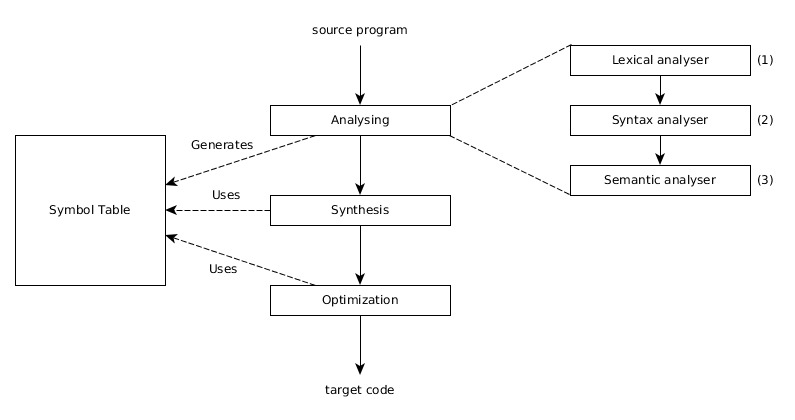
\includegraphics[scale=0.3]{./img/phase_of_compiler.jpg}\\
    \textit{Figure 1~-~Compilation phases.}
  \end{center}
  
\section{Implementation of the lexical analyser}

\end{document}
